% arara: pdflatex: { synctex: on }
% arara: bibtex
% arara: pdflatex: { synctex: on }
% arara: pdflatex: { synctex: on }

\documentclass[letterpaper, 10 pt, conference]{ieeeconf}  % Comment this line out if you need a4paper
%\documentclass{article}  % Comment this line out if you need a4paper

%\documentclass[a4paper, 10pt, conference]{ieeeconf}      % Use this line for a4 paper

\IEEEoverridecommandlockouts                              % This command is only needed if
                                                          % you want to use the \thanks command

\overrideIEEEmargins                                      % Needed to meet printer requirements.

% See the \addtolength command later in the file to balance the column lengths
% on the last page of the document

% The following packages can be found on http:\\www.ctan.org
\usepackage{graphics} % for pdf, bitmapped graphics files
\usepackage{epsfig} % for postscript graphics files
\usepackage{mathptmx} % assumes new font selection scheme installed
\usepackage{times} % assumes new font selection scheme installed
\usepackage{mathtools} % assumes amsmath package installed
\usepackage{amssymb}  % assumes amsmath package installed
\usepackage{amsmath}
\usepackage{tikz}
\usepackage{MnSymbol}
\usetikzlibrary{positioning,graphs,calc,backgrounds,fit,arrows,patterns,shapes}
\usepackage{tabulary}
\usepackage{hyperref}
\usepackage{cite}


\newcommand{\hvec}{\overset{\rightharpoonup}}
\newcommand{\argmin}{\arg\!\min}
\newcommand{\norm}[1]{\left\lVert#1\right\rVert}
\newcommand{\quotes}[1]{``#1''}
%\usepackage{biber}

%\title{\LARGE \bf
%Reactive Obstacle Avoidance Plugin (ROAP)\\ for Computationally-Constrained MAVs
%}
\title{\LARGE \bf  Tightly-Coupled Visual-Inertial Relative Navigation}

\author{James Jackson}% <-this % stops a space


\begin{document}

\maketitle
\thispagestyle{empty}
\pagestyle{empty}

\section{Derivation}

\subsection{State Definition}

\newcommand{\bx}{\mathbf{x}}
\newcommand{\xdot}{\dot{\mathbf{x}}}
\newcommand{\xhat}{\hat{\mathbf{x}}}
\newcommand{\xtilde}{\tilde{\mathbf{x}}}
\newcommand{\pos}{\mathbf{p}}
\newcommand{\pdot}{\dot{\mathbf{p}}}
\newcommand{\vel}{\mathbf{v}}
\newcommand{\vdot}{\dot{\mathbf{v}}}
\newcommand{\quat}{\mathbf{q}}
\newcommand{\balpha}{\mathbf{\alpha}}
\newcommand{\bbeta}{\mathbf{\beta}}
\newcommand{\qdot}{\dot{\mathbf{q}}}
\newcommand{\badot}{\dot{\mathbf{\alpha}}}
\newcommand{\bbdot}{\dot{\mathbf{\beta}}}
\newcommand{\bmu}{\mathbf{\mu}}
\newcommand{\bmudot}{\dot{\mathbf{\mu}}}
\newcommand{\bomega}{\mathbf{\omega}}
\newcommand{\crs}{_\times}
\newcommand{\bxi}{\mathbf{\xi}}
\newcommand{\bu}{\mathbf{u}}
\newcommand{\bn}{\mathbf{n}}
\newcommand{\bnu}{\mathbf{\nu}}

\newcommand{\acc}{\mathbf{a}}
\newcommand{\grav}{\mathbf{g}}

\newcommand{\bigR}{\mathbb{R}}
\newcommand{\bigS}{S}

\newcommand{\btheta}{\mathbf{\theta}}
\newcommand{\atan}{\textrm{atan}}

\newcommand{\sV}{\mathcal{V}}

\newcommand{\ihat}{\hat{\mathbf{i}}}
\newcommand{\jhat}{\hat{\mathbf{j}}}
\newcommand{\khat}{\hat{\mathbf{k}}}


\begin{equation}
\begin{aligned}
	\bx = (\pos, \vel, \quat, \balpha, \bbeta, \bmu_0,  \dots, \bmu_N, \rho_0, \dots, \rho_N)
\end{aligned}
\end{equation}

\subsection{3D Rotation Representation}
Because rotations are a part of $SO(3)$ with group operator $\otimes$, there is no notion of addition or subtraction, and therefore no differentiation.  Since $SO(3)$ is a Lie, group, we can instead map to the Lie Algebra $\mathfrak{so}(3): \btheta \in \bigR^{3}$  We will parameterize rotations as quaternions where $\quat \in \bigR^4$ and is overparameterized.  We then define the exponential map that maps from $SO(3)$ to $\mathfrak{so}(3)$

\begin{equation}
\begin{aligned}
	\log: \quad SO(3) &\rightarrow \bigR^3, \\
	\quat &\mapsto \log(\quat) = \btheta \\ \\
	\exp: \quad \bigR^3 &\rightarrow SO(3), \\
	\btheta &\mapsto \exp(\btheta) = \quat 
\end{aligned}
\end{equation}

where

\begin{equation}
\begin{aligned}
	\exp(\btheta) &= \begin{bmatrix} \cos \norm{\btheta} \\ \textrm{sinc} \norm{\btheta} \btheta \end{bmatrix} \\
	\log\left(\begin{bmatrix} w \\ \vel \end{bmatrix} \right) &=  \begin{cases} 
														0 & \vel = 0  \\
														\dfrac{\atan\left(\tfrac{\norm{\vel}}{w}\right)}{\norm{\vel}}\vel & \vel \neq 0, \; w = 0 \\ 
														\pm \dfrac{\tfrac{\pi}{2}}{\norm{\vel}}\vel & w = 0
													\end{cases}
\end{aligned}
\end{equation}

We will define a helpful syntax that will allow us to work with members of the Lie group similar to the way we work with vectors $\boxplus$ and $\boxminus$.  These operators will act intuitively like the $+$ and $-$ operators of a vector space, but will use the exponential map to ensure we do not leave the manifold of the group.


\begin{equation}
\begin{aligned}
	\quat \boxplus \btheta &= \quat \otimes \exp\left(\tfrac{\btheta}{2}\right) \\
	\quat \boxminus \mathbf{p} &= 2 \log\left(\mathbf{p}^{-1} \otimes \quat\right)
\end{aligned}
\end{equation}

Where $\otimes$ is standard quaternion multiplication.


\subsection{Bearing Vector Parameterization}

We will use quaternions $\bmu_i$ to represent the rotation between the camera frame $z$-axis and the normal vector pointing at the feature in the camera frame.  Similarly to representing attitude using the quaternion $\quat$, $\bmu_i$ is over-parameterized.  The difference is that the space of all $\bmu_i$ is actually defined over the unit sphere. $\bigS^2$ and there are only 2 degrees of freedom, in this space as opposed to 3 in $\bigR^3$.

To get the unit vector to the feature, we employ the following quantity

\begin{equation}
\begin{aligned}
	\bn(\bmu) := \bmu(\khat_\sV) \in \bigS^2 \subset \bigR^3
\end{aligned}
\end{equation}

Where $\ihat_\sV, \jhat_\sV, \khat_\sV$ are the unit basis vectors of the camera frame.

However, because of the way that $\bigS^2$ works, we can reduce the dimensionality even further by considering a vector in $\bigR^2$ which describes the axis upon which $\bmu$ operates, scaled by the angle of rotation (See Figure~\ref{fig:unit_vector}).  To get the unit vector in this direction, we employ the projection matrix $N$

\begin{equation}
\begin{aligned}
	N(\bmu) := \begin{bmatrix} \bmu(\ihat_\sV) & \bmu(\jhat) \end{bmatrix} \in \bigR^{3\times2}
\end{aligned}
\end{equation}

on the and scale it by the angle of rotation from $\bmu$

\begin{equation}
	\phi = 2 \textrm{acos} (\bmu_w)
\end{equation}


\begin{figure}
	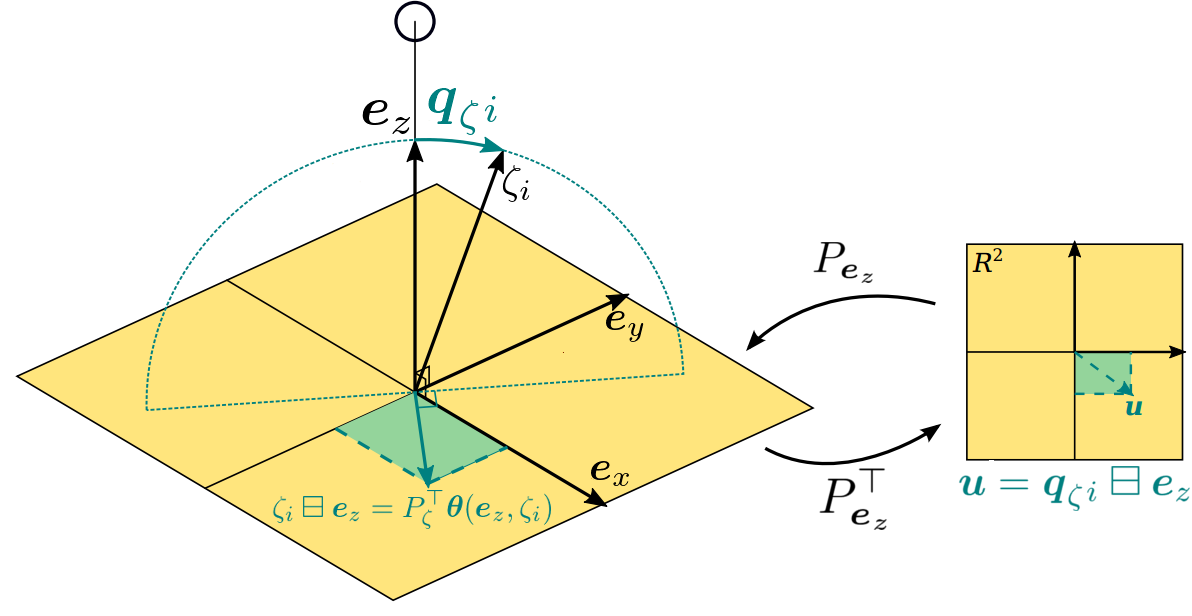
\includegraphics[width=\columnwidth]{figures/unit_vector_picture.png}
	\caption{Illustration of unit vector parameterization}
	\label{fig:unit_vector}
\end{figure}




To deal with this manifold, we will use the following $\boxplus$ and $\boxminus$ operators and mappings.

\begin{equation}
\begin{aligned}
	\boxplus : SO(3) \times \bigR^2 &\rightarrow SO(3), \\
	\bmu, \bu &\mapsto \exp(N(\bmu)\bu) \otimes \bmu \\ \\
	\boxminus : SO(3) \times SO(3) &\rightarrow \bigR^2, \\
	\bnu, \bmu &\mapsto N(\bmu)^\top \left( \bmu \boxminus \bnu \right)
	\end{aligned}
\end{equation}





\subsection{Dynamics}

Now that we have defined the parameterization for the non-vector states, we are ready to define the dynamics of our system:

\begin{equation}
\begin{aligned}
	\pdot &= -\bomega\crs \pos + \vel + \bxi_\pos \\
	\vdot &= -\bomega\crs \vel + \acc + R(\quat)^{-1}(\grav) \\
	\qdot &= -R(\quat)\bomega \\
	\badot &= \bxi_\balpha \\
	\bbdot &= \bxi_\bbeta \\
	\dot{\bmu_i} &= N^\top(\bmu_i)\bomega_\sV - \begin{bmatrix} 0 & 1 \\ -1 & 0 \end{bmatrix}N^\top(\mu_i)\dfrac{\vel_\sV}{d(\rho_i)} + \bxi_{\bmu_i} \\
	\dot{\rho}_i &= -\bmu_i^\top \dfrac{\vel_\sV}{d'(\rho_i)} + \bxi_{\rho_i}
\end{aligned}
\end{equation}

These dynamics are used to propagate the reference state $\xhat$, while the following dynamics are used to propagate the error state $\xtilde$

\begin{equation}
\begin{aligned}
	\pdot &= -\bomega\crs \pos + \vel\\
	\vdot &= -\bomega\crs \vel + \acc + R(\quat)^{-1}(\grav) \\
	\qdot &= -R(\quat)\bomega \\
	\badot &= 0\\
	\bbdot &= 0 \\
	\dot{\bmu_i} &= N^\top(\bmu_i)\bomega_\sV - \begin{bmatrix} 0 & 1 \\ -1 & 0 \end{bmatrix}N^\top(\mu_i)\dfrac{\vel_\sV}{d(\rho_i)} \\
	\dot{\rho}_i &= -\bmu_i^\top \dfrac{\vel_\sV}{d'(\rho_i)}
\end{aligned}
\end{equation}







% \bibliography{library}
% \bibliographystyle{ieeetr}

\end{document}


%%%%%%%%%%%%%%%%%%%%%%%%%%%%%%%%%%%%%%%%%%%%%%%%%%%%%%%%%%%%%%%%%%%%%%%%%%%%%

% SAVED STUFF






%new document

